\section{\systemname{}: Visual Search for Programming Solutions}

\systemname{} helps users select suitable code examples by enabling visual inspection of code-text ratio, inspection and localization of common classes, and comparison of similar examples.
We describe the design of visualizations to help these tasks.
This includes content-colored columns, class frequency charts with brushing and linking to the source examples, and a snippet bank.
We build the UI for \systemname{} to encourage rapid systematic skim over many examples and decrease the time of link-based context switches.

\subsection{Code Example Columns}

We expect some users to look for text-heavy explanatory documents like tutorials, and others to look for short segments of code to insert into their programs.
We encode different types of content like source code, plaintext, and code comments, as different colored blocks.
One block corresponds to one sentence of plaintext or one line of code.
These blocks are stacked from top to bottom to maintain the metaphor of a vertical programming example text from StackOverflow.
An answer converted to the visual space of \systemname{} is shown in Figure~\ref{fig:bar_conversion}.

\begin{figure}
 \centering
 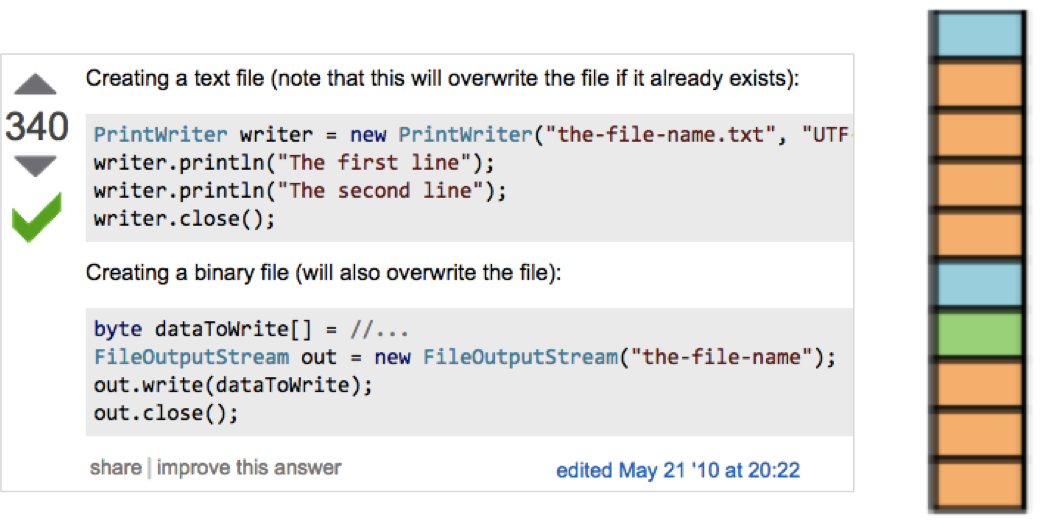
\includegraphics[width=.9\columnwidth]{figures/so_to_ss}
 \caption{A StackOverflow answer and its representation as a column in \systemname{} search results.
    Plaintext sentences become blue blocks, code lines orange blocks, and inline comments green blocks.
    By inspecting the resulting column, one can see that the example begins with short plaintext, demonstrates the idea with code, provides additional text, and ends with another segment of code.}
 \label{fig:bar_conversion}
\end{figure}

Bars are packed horizontally for users to rapidly assess which programming examples contain the most content overall (see Figure~\ref{fig:bar_length}).
The vertical window size fits around 80\% of the answers we viewed during our own use of the tool. This enables users to view the full column of most displayed results.

\begin{figure}
 \centering
 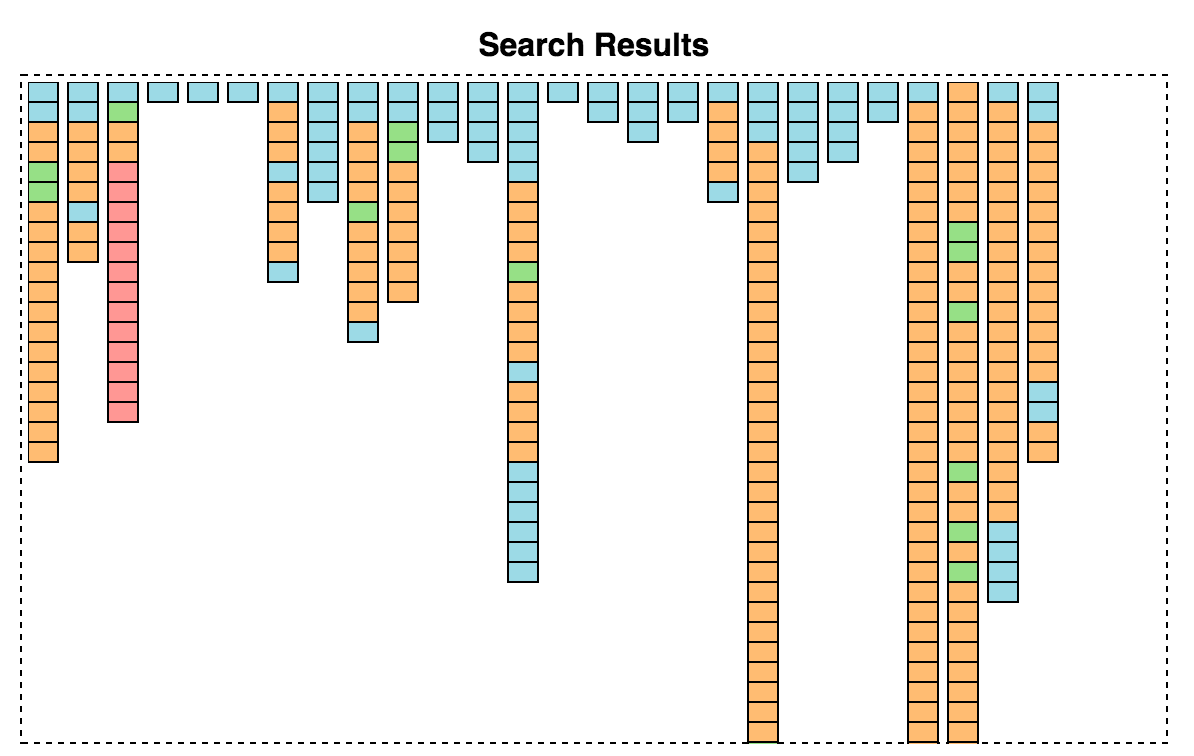
\includegraphics[width=.9\columnwidth]{figures/bars_unaltered}
 \caption{A vertical bar represents an answer from StackOverflow.  
 In this image, you can see 13 explanatory answers made completely of plaintext and several examples with over 20 lines of code.}
 \label{fig:bar_length}
\end{figure}

To help users quickly locate search results that match their content preference, we provide a simple sorting interface.
Using a dropdown menu (Figure~\ref{fig:sort_pane}), users can choose whether to sort search results and their representative columns by total example length (Figure~\ref{fig:length_sorted}), lines of code, sentences of plaintext (Figure~\ref{fig:text_sorted}), votes or author reputation.

\begin{figure}[t]
    \centering
    \begin{subfigure}[b]{0.45\columnwidth}
        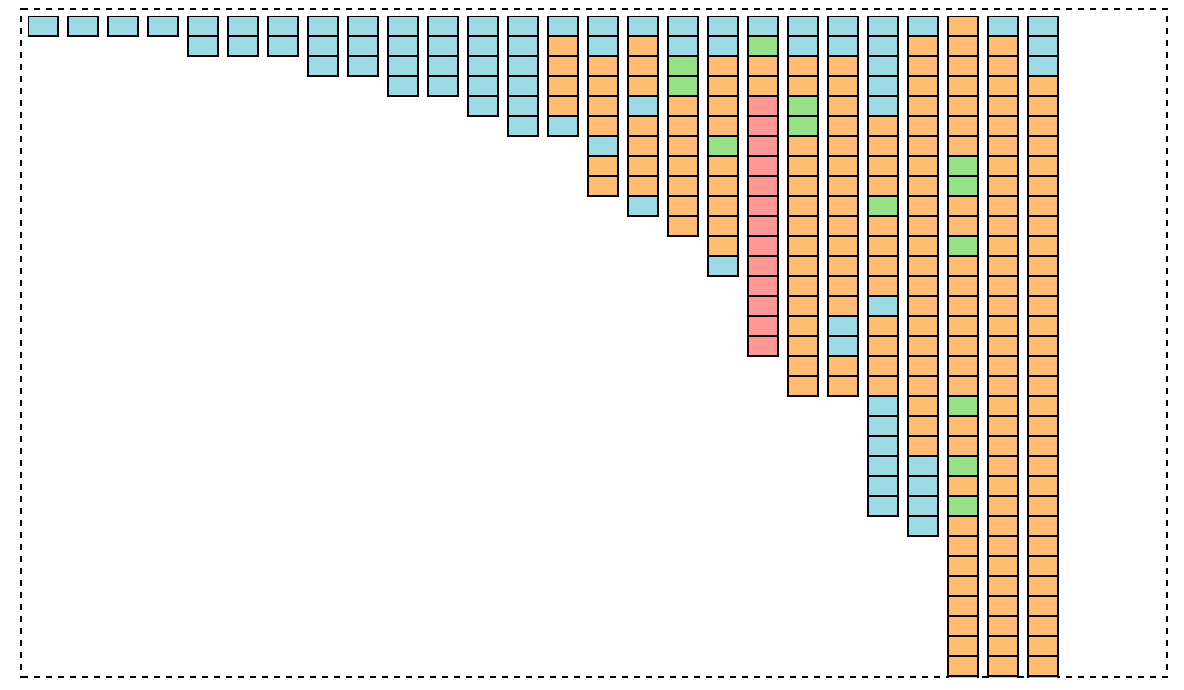
\includegraphics[width=\textwidth]{figures/length_sorted}
        \caption{Sorting by total content length.}
        \label{fig:length_sorted}
    \end{subfigure}
    \begin{subfigure}[b]{0.45\columnwidth}
        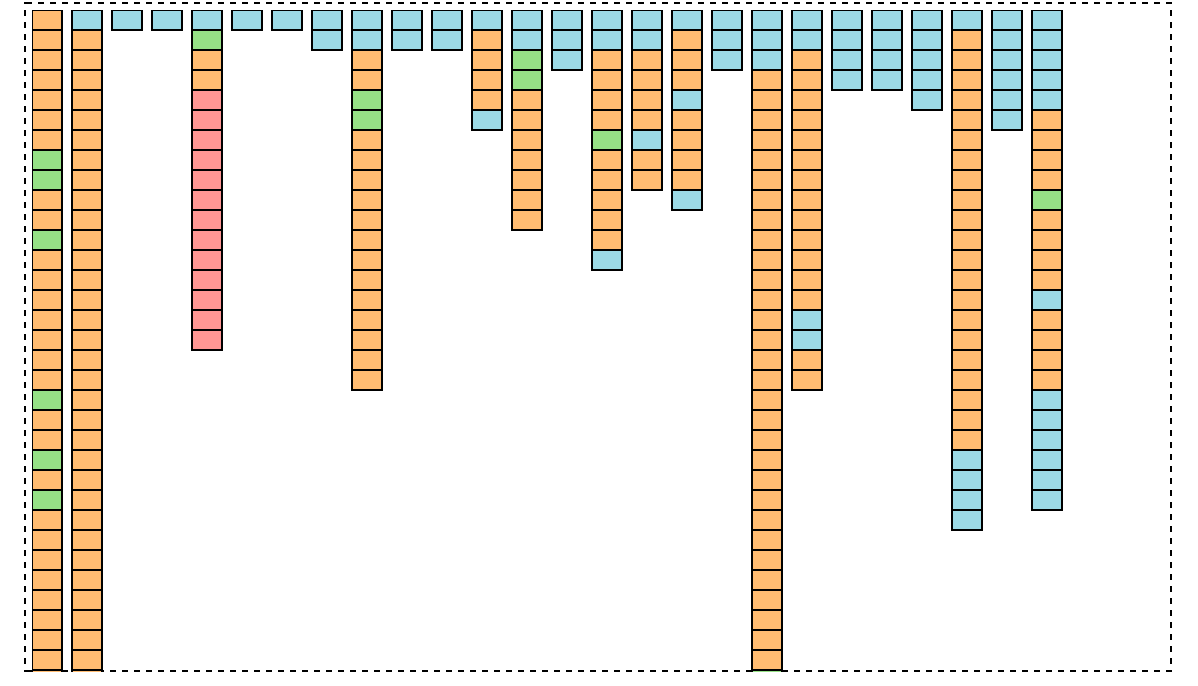
\includegraphics[width=\textwidth]{figures/text_sorted}
        \caption{Sorting by plaintext sentences.}
        \label{fig:text_sorted}
    \end{subfigure}
    \begin{subfigure}[b]{0.3\columnwidth}
        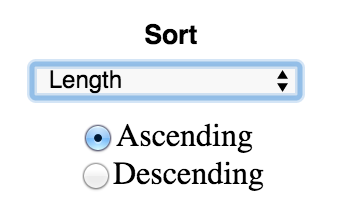
\includegraphics[width=\textwidth]{figures/sort_pane}
        \caption{Sorting widget.}
        \label{fig:sort_pane}
    \end{subfigure}
    \caption{Sorting code examples by content type (in this case, total content and plaintext sentence count) in \systemname{}.}
\end{figure}

\subsection{Source Text Preview Pane}

We enable users to inspect the source text of examples for two reasons.
First, they must determine if the solution the bar presents is relevant to their query.
Second, if the example is relevant, users will want to copy text from the example into their own programs.

\systemname{} enables users to skim the source of dozens of examples across multiple questions with small movements of the mouse.
By positioning the cursor over a block of an example, the preview pane highlights that block of code amidst 10 - 20 blocks of surrounding context (Figure~\ref{fig:preview}).
We assumed users would be predominantly scrolling down through examples.
Therefore, we saved 30\% of the preview pane's verticals space to show blocks above, and 70\% for blocks below the focused block.
The window animates vertical scrolling between different blocks in the same example.
Users can shift their focus to the source text of another example by moving the mouse horizontally to another example column.

\begin{figure}[b]
 \centering
 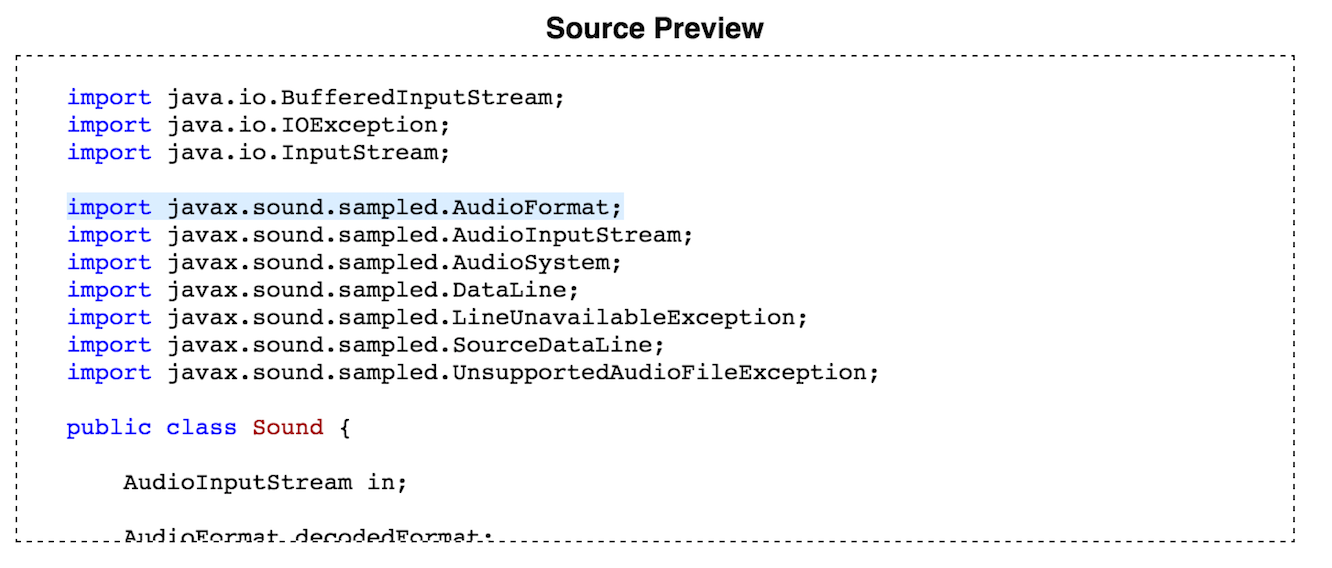
\includegraphics[width=\columnwidth]{figures/preview_pane_selected}
 \caption{The preview pane shows the source text of an example a user is hovering over.
 The pane highlights the currently hovered block in pale blue.
 The focused block is surrounded by text from the blocks immediately preceding and following it to provide the user with context.}
 \label{fig:preview}
\end{figure}

We used a preview window instead of tooltip-based inspection due to space constraints.
A horizontal space of around 60 characters shows source code content without frequent line wrap or horizontal scrolling.
A vertical space of 10 - 15 lines shows source code before and after the highlighted region or several sentences of explanatory text that come directly before or after.
A tooltip showing 10 lines of text 60 characters would be massive or have a small font.
To avoid occluding other bars of text, we opted to decouple the preview pane from the mouse position, and place it in a separate region at the top of the screen.

\subsection{Class and Concept Inspection}

We show users commonly used libraries in code examples to direct them to corresponding documentation prior to using the examples.
We provided details about classes and concepts which were most used across all examples with easy access to the regions of code that used those classes and concepts.

First, we present a markup pane with bar charts that provide a quick visual description of what material would be helpful for a user to examine before examining the search results (Figure~\ref{fig:markup_pane}).
Bar charts show the frequency of Java classes and concepts (objects, functions, loops, etc.) ordered from greatest number of occurrences to least.

\begin{figure}[b]
 \centering
 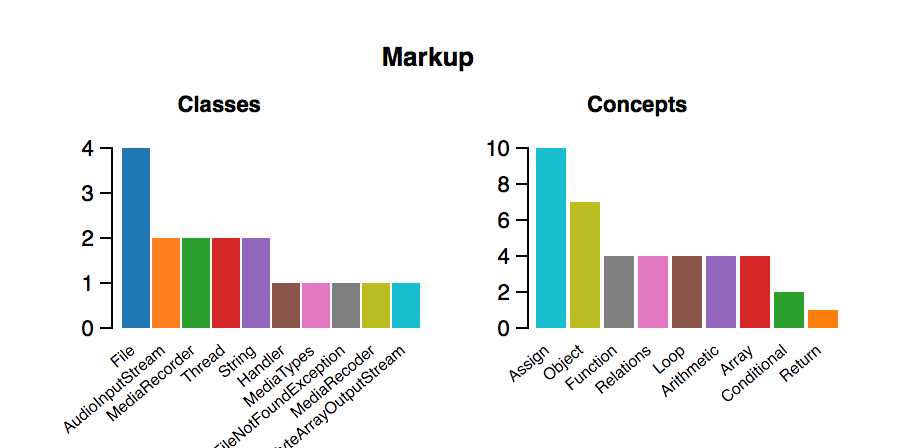
\includegraphics[width=\columnwidth]{figures/markup_bar}
 \caption{The Markup pane presents which dependencies and code techniques are used most often.  By clicking on bars, users highlight all blocks that use that class or concept.  Labels for the class bar chart link to Java API documentation.}
 \label{fig:markup_pane}
\end{figure}

Second, we enable users to gain additional background knowledge on these libraries quickly.
Labels for classes link to the Java API for access to more comprehensive documentation.

Third, users can mark regions of examples that use of a class, to find alternate approaches to leveraging the same classes and typical modes of use.
By hovering over a library dependency in the summary pane, all code examples that use that dependency are highlighted in the search results.
By clicking on one of those library dependencies in the markup pane, users flag all blocks of all examples that instantiate that class or use that concept.
Users can then visually filter for or exclude examples that contain that dependency.

Colors of class and concept markers have greater saturation than the colors used to mark the block content to make them stand out against the blocks they mark.
Classes and concept markers are colored using the Tableau 10 colors and assigned based on frequency of class or concept occurence.

\subsection{Saving and Comparing Code Examples}

In our preliminary study, programmers revisited old code and kept many tabs open.
We introduce a snippets bank for preserving past potentially relevant code.
This concentrates all relevant code in one location for skimming through past results.

Users click and drag over blocks of code in a single example that they want to keep (Figure~\ref{fig:selection_regions}).
After releasing the mouse, a new snippet is pushed to the top of the \emph{Snippets} stack (Figure~\ref{fig:snippets}).
This ensures that the most recent results are instantly viewable.
Users can edit titles of snippets to later recall why they saved the snippet.
Individual snippets and be collapsed and expanded to enable a user to open several examples for direct comparison.

\begin{figure}
    \centering
    \begin{subfigure}[b]{0.8\columnwidth}
        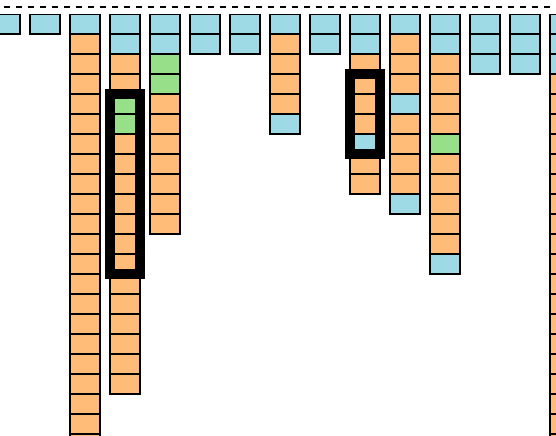
\includegraphics[width=\textwidth]{figures/selection_regions}
        \caption{User clicks and drags over blocks of text.}
        \label{fig:selection_regions}
    \end{subfigure}
    \bigskip
    \begin{subfigure}[b]{0.9\columnwidth}
        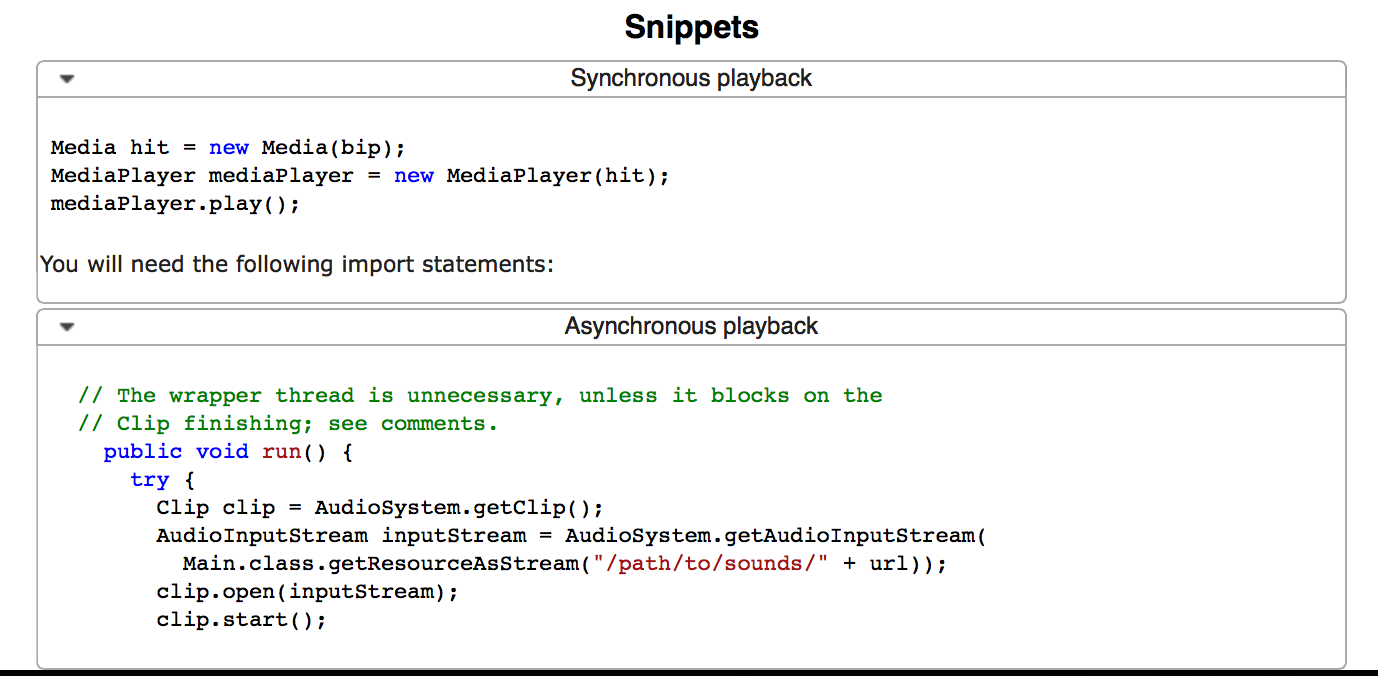
\includegraphics[width=\textwidth]{figures/snippets}
        \caption{Source text from the selected regions are added to the snippets pane for saving multiple relevant results for later inspection.}
        \label{fig:snippets}
    \end{subfigure}
    \caption{By clicking and dragging over a search result column, users create example snippets and store them in the snippet bank.}
\end{figure}

In the future, we will provide a way to sort, edit, combine and markup snippets.
We will also link snippets visually to the search columns they were extracted from.

\subsection{Iterative Search UI}

The utility of \systemname{} requires that users have multiple examples to skim through.
During search tasks, this is not always the case.
Some StackOverflow questions have only one answer.
We also observed users end their search after considering only one relevant question and answer.

To make \systemname{} pertinent for solving programming problems with multiple examples, we developed search UI elements to help users discover many relevant answers prior to examining search results.
After a user performs a query in the search box at the top of the page, we fetch the 20 relevant \emph{questions} from StackOverflow.
We list the title of each question in a list shown to the user (Figure~\ref{fig:question_selection}).
The user selects questions relevant to their query.
For example, for a query ``play audio'', a user might select questions titled \emph{Java audio playing solution?}, \emph{Play audio file in java}, \emph{Playing audio in Java}, and \emph{Reading and playing audio file}.
\systemname{} populates the search results with every answer to these questions.

\begin{figure}
    \centering
    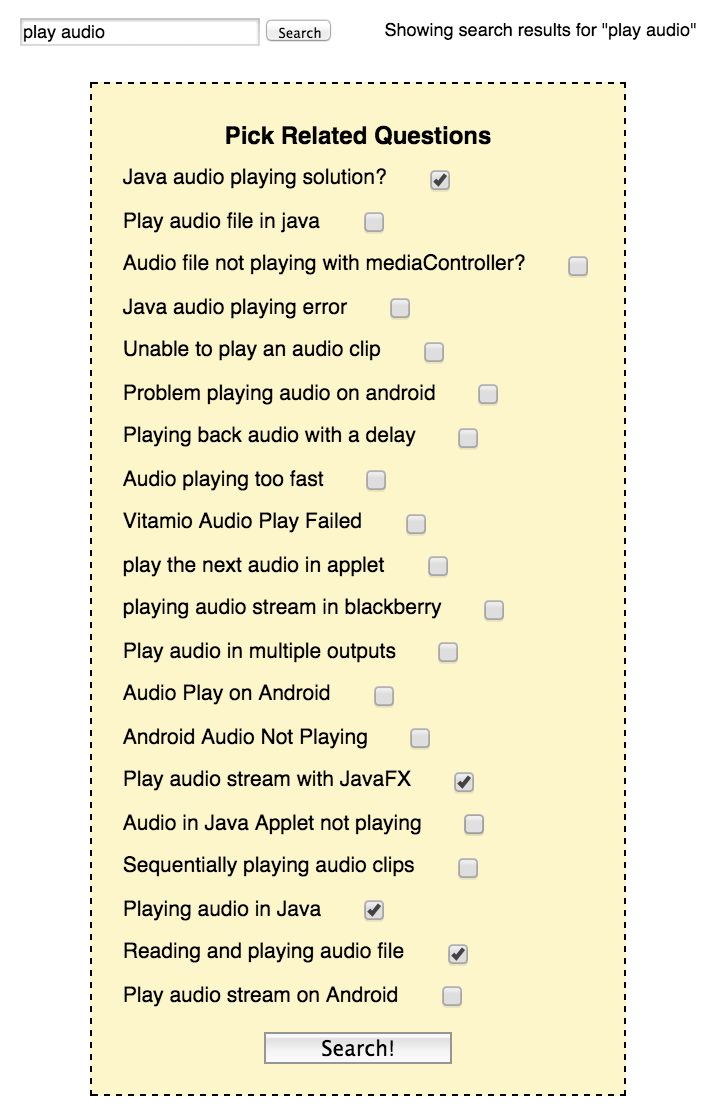
\includegraphics[width=.6\columnwidth]{figures/question_selection.png}
    \caption{Users select questions related to their query in the question selection popup after each query.
    By selecting related questions, users populate the search results with relevant answers.}
    \label{fig:question_selection}
\end{figure}

During later queries, \systemname{} maintains all snippets that users have selected from past queries.
In this way, users can compare examples between initial and later, refined queries.
They can also store snippets from multiple steps in a sequence that will eventually form a longer program.

At this point, users cannot view the questions that answers address.
Future work could explore how to represent questions in our interface as multiple answers share the same question.
In addition, question selection could be augmented by showing excerpts from the question body and counts of answers to help users both assess question relevance and breadth of answers covered by their selection.